Xampp merupakan singkatan dari X (empat sistem operasi apapun), Apache, Mysql, PHP, dan Perl. Xampp adalah tool yang menyediakan paket perangkat lunak dalam satu buah paket. Dalam paket Xampp sudah terdapat Apache (web server), Mysql (database), PHP (server side scripting), Perl ,FTP server, PhpMyAdmin dan berbagai pustaka bantu lainya. XAMPP adalah perangkat lunak bebas, yang mendukung banyak sistem operasi, merupakan kompilasi dari beberapa program \cite{sugiarto2019aplikasi}.

\section{Tutorial Install Xampp}
\begin{enumerate}
    \item Download terlebih dahulu aplikasi Xampp di https://www.apachefriends.org/index.html, download sesuai sistem operasi yang anda gunakan, pada tutorial kali ini saya akan melakukan instalasi XAMPP di Windows 10.
    
	\item Setelah download aplikasi, lakukan instalasi XAMPP, dengan cara klik kanan pada file instalasi kemudian pilih Open.
		\begin{figure}[!htbp]
    		\centering
    		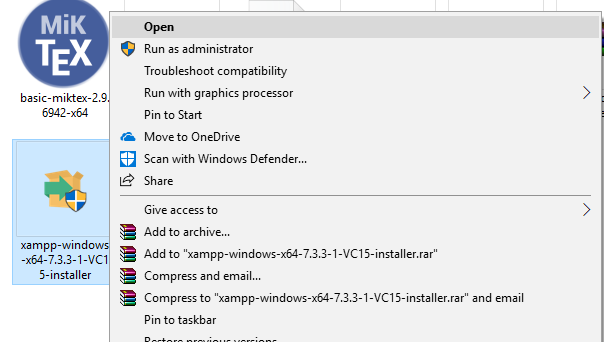
\includegraphics[width=0.5\textwidth]{figures/Xampp2.png}
    		\label{Xampp2}
		\end{figure}
		
	\item Jika pada saat melakukan instalasi muncul peringatan yang bertujuan untuk memastikan apakah Anda akan menginstal aplikasi ini, Silakan klik Ok/Yes untuk melanjutkan instalasi.
		\begin{figure}[!htbp]
    		\centering
    		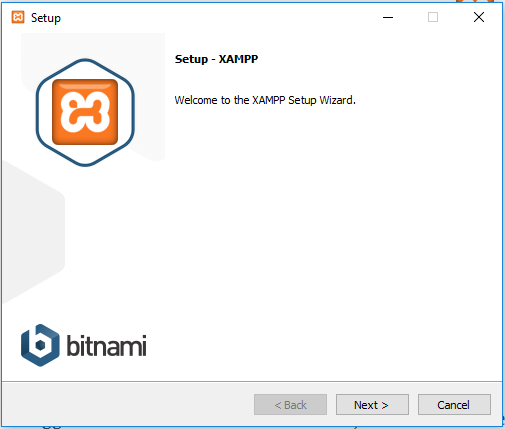
\includegraphics[width=0.5\textwidth]{figures/Xampp3.PNG}
    		\label{Xampp3}
		\end{figure}
		
	\item Klik next untuk melanjutkan, kemudian akan tampil pilihan aplikasi apa yang akan Anda install dan tidak ingin Anda install.
		\begin{figure}[!htbp]
    		\centering
    		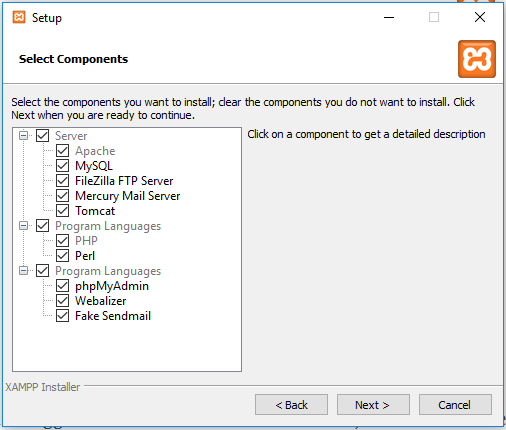
\includegraphics[width=0.5\textwidth]{figures/Xampp4.PNG}
    		\label{Xampp4}
		\end{figure}
		
	\item Tahap selanjutnya adalah memilih folder dimana lokasi instalasi xampp akan disimpan.
		\begin{figure}[!htbp]
    		\centering
    		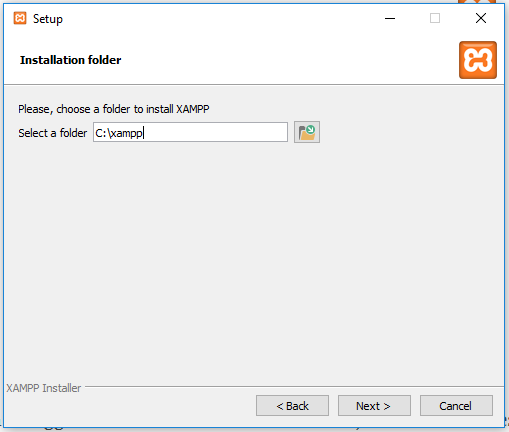
\includegraphics[width=0.5\textwidth]{figures/Xampp5.PNG}
    		\label{Xampp5}
		\end{figure}
		
	\item Silakan hilangkan centang pada “Learn more about Bitnami for XAMPP”, kemudian klik Next.
		\begin{figure}[!htbp]
    		\centering
    		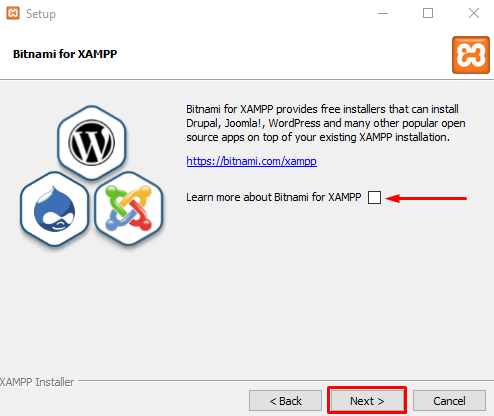
\includegraphics[width=0.5\textwidth]{figures/Xampp6.png}
    		\label{Xampp6}
		\end{figure}
		
	\item Klik next untuk malnjutkan ke proses instalasi xampp.
		\begin{figure}[!htbp]
    		\centering
    		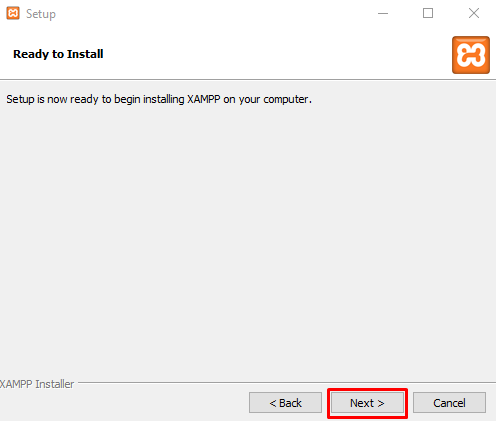
\includegraphics[width=0.5\textwidth]{figures/Xampp7.png}
    		\label{Xampp7}
		\end{figure}
		
	\item Apabila aplikasi sudah terinstal maka akan tampil pertanyaan mengenai apakah Anda ingin langsung menjalankan control panel. Pastikan pilihan tersebut sudah tercentang, kemudian klik tombol Finish.
		\begin{figure}[!htbp]
    		\centering
    		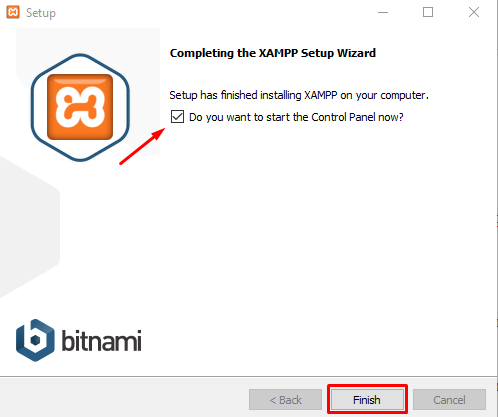
\includegraphics[width=0.5\textwidth]{figures/Xampp8.png}
    		\label{Xampp8}
		\end{figure}
		
	\item Control panel akan muncul otomatis, tapi jika Anda tidak mencentang pilihan di halaman sebelumnya, maka Anda perlu membuka langsung control panel melalui start menu atau folder XAMPP di komputer Anda.
	
	\item Apabila control panel sudah muncul dan terlihat seperti gambar \ref{Xampp9}, maka proses instalasi Xampp berhasil.
		\begin{figure}[!htbp]
    		\centering
    		\caption{Control Panel Xampp}
    		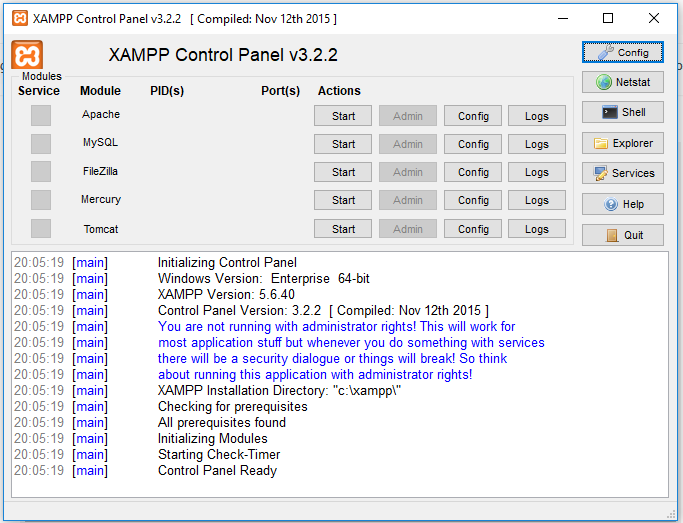
\includegraphics[width=0.5\textwidth]{figures/Xampp9.PNG}
    		\label{Xampp9}
		\end{figure}
\end{enumerate}

\section{Mengatasi Error Pada Xampp}
Hal yang menjadi penyebab utama kenapa tampil error pada XAMPP biasanya disebabkan aplikasi lain pada komputer Anda menggunakan port 80 atau 443, dimana port tersebut digunakan oleh Apache dan MySQL. Berikut cara mengatasi error pada xampp:
\begin{enumerate}
    \item Klik Start, kemudian ketikkan “services.msc” pilih Services yang ada di bagian Best match.
    \item Scrol ke bawah, pada bagian World Wide Web Publishing Service klik kanan dan pilih Stop.
    \item Silakan close XAMPP, kemudian buka kembali dan jalankan Apache dan MySQL pada XAMPP.
\end{enumerate}

Jika langkah yang Anda lakukan tidak berhasil mengatasi masalah yang dihadapi atau tidak menemukan World Wide Web Publishing, silakan lakukan langkah di bawah ini:
\begin{enumerate}
    \item Buka control panel melalui tombol start yang ada pada pojok kiri bawah
    
    \item Kemudian pilih system and security
		\begin{figure}[!htbp]
    		\centering
    		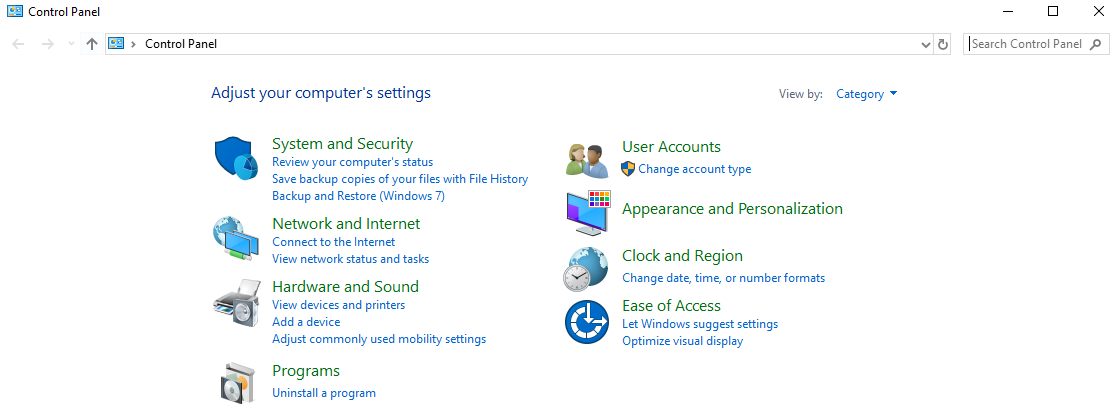
\includegraphics[width=0.5\textwidth]{figures/Xampp12.PNG}
    		\label{Xampp12}
		\end{figure}
		
	\item Pilih windows defender firewall
		\begin{figure}[!htbp]
    		\centering
    		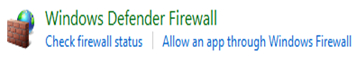
\includegraphics[width=0.5\textwidth]{figures/Xampp13.PNG}
    		\label{Xampp13}
		\end{figure}
		
	\item Pilih advanced settings
		\begin{figure}[!htbp]
    		\centering
    		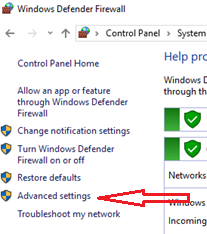
\includegraphics[width=0.5\textwidth]{figures/Xampp14.PNG}
    		\label{Xampp14}
		\end{figure}
		
	\item Klik Inbound dan klik kanan kemudian pilih New Rule, dapat dilihat seperti pada gambar dibawah
		\begin{figure}[!htbp]
    		\centering
    		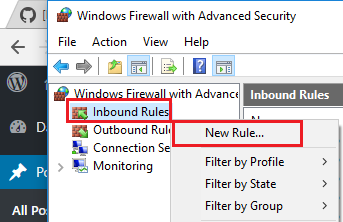
\includegraphics[width=0.4\textwidth]{figures/Xampp15.png}
    		\label{Xampp15}
		\end{figure}
		
	\item Pilih Port dan tekan tombol Next, kemudian pada kolom Specific Ports isi dengan 80, 443 kemudian klik Next.
		\begin{figure}[!htbp]
    		\centering
    		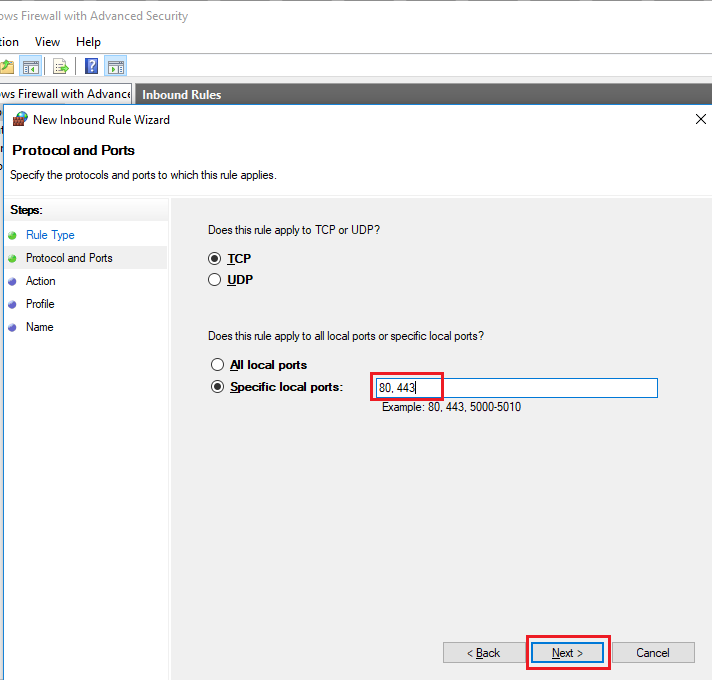
\includegraphics[width=0.5\textwidth]{figures/Xampp16.png}
    		\label{Xampp16}
		\end{figure}
		
	\item Centang Allow the Connection kemudian klik Next
		\begin{figure}[!htbp]
    		\centering
    		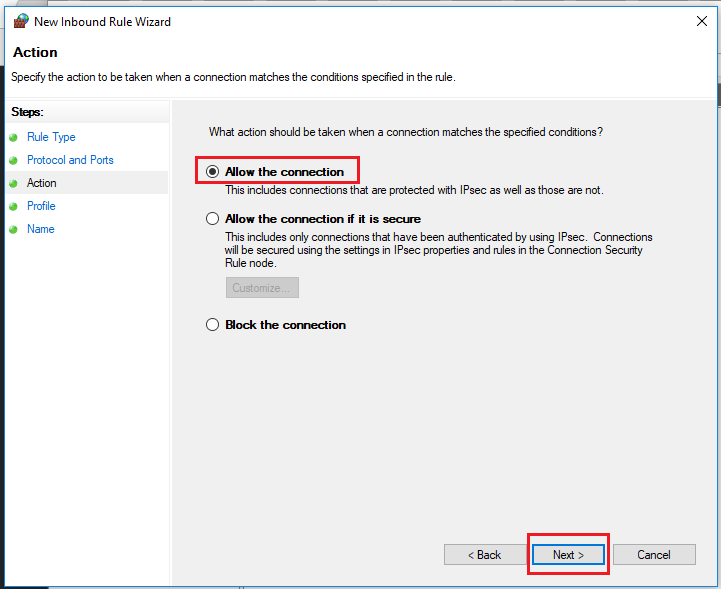
\includegraphics[width=0.5\textwidth]{figures/Xampp17.png}
    		\label{Xampp17}
		\end{figure}
		
	\item Pastikan semua pilihan dicentang seperti pada gambar dibawah, kemudian klik Next
		\begin{figure}[!htbp]
    		\centering
    		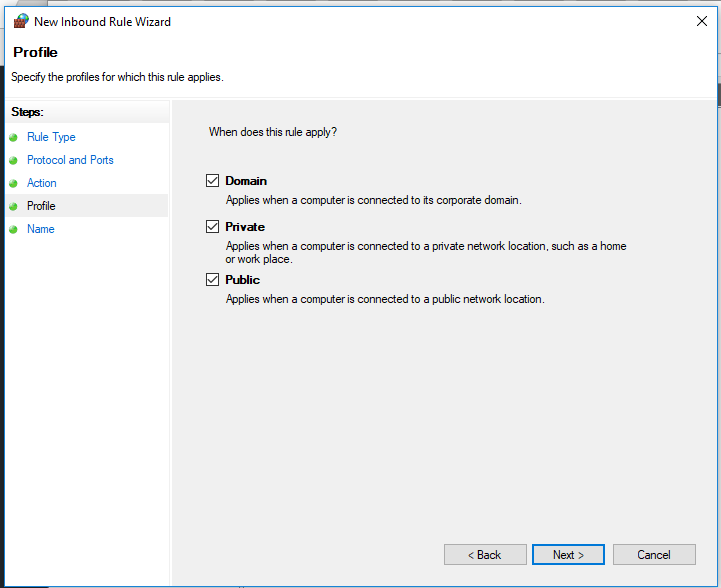
\includegraphics[width=0.5\textwidth]{figures/Xampp18.png}
    		\label{Xampp18}
		\end{figure}
		
	\item Masukkan lokal1 pada kolom name, kemudian klik Finish
		\begin{figure}[!htbp]
    		\centering
    		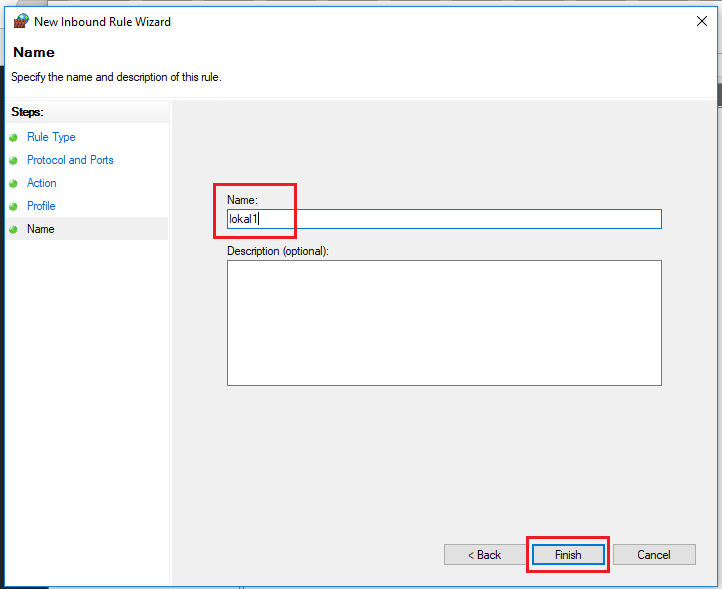
\includegraphics[width=0.5\textwidth]{figures/Xampp19.png}
    		\label{Xampp19}
		\end{figure}
		
	\item Ulangi kembali langkah 1 sampai 6, untuk langkah 6 isi dengan lokal2, kemudian klik Finish
	
	\item Restart komputer Anda 
\end{enumerate}